
\section{正\trGenus{}\trCurve{}产生的经典几何}

后文我们会用到下面的\trhProposition{}与\trhCorollary，而我们也以此为由头，从现代的立场重访一些非常经典的几何。

\textbf{19.4.1.\ \trhProposition。}\ ——\ \emph{回想本章的\trStandingHypothesis（\S19.2.1）：$C$ 是域 $k$ 上一条\trProjective、几何正则、\trGeometricallyIntegral{}的\trCurve。设 $C$ 不同构于 $\mathbb{P}^1_k$（对其\trGenus{}不作任何假设），且 $\mathscr{L}$ 是一个\trDegree{}为 $1$ 的\trInvertibleSheaf。则 $h^0(C,\mathscr{L})<2$。}

\emph{证明。}\quad 我们本可以仿照\mbox{命题~19.3.1} 来证明它（读者也不妨一试）。但我们改为「徒手」证明，因为\mbox{命题~19.3.1} 要用到\trSerreDuality，而我们要到第 29 章才会证明它（况且它也很难），我们想强调：这个结果用不着\trSerreDuality。此外，有些读者或许从未读过任何关于\trSerreDuality{}的内容，也照样能读懂这个论证。

假设陈述不真，并设 $s_1$ 与 $s_2$ 为两个（相互独立的）\trSection。由于 $s_i$ 的零点\trDivisor{}的\trDegree{}就是 $\mathscr{L}$ 的\trDegree，故二者各自在单独一点 $p_i$ 处消失（消失到 $1$ 阶）。

现在，$p_1\ne p_2$。（否则，若 $p_1=p_2$，则 $s_1/s_2$ 既无极点又无零点，于是由代数\trHartogs{}引理——见 \S13.5.20——它是一个可逆函数，而借助 \S11.4.7（在基变换到 $\bar{k}$ 之后）它又是一个常值函数。这与 $s_1$ 与 $s_2$ 的线性无关性矛盾。）

于是 $s_1$ 与 $s_2$ 生成一个\trBasePointFree\trLinearSystem，从而我们便有一个诱导出的\trMorphism{} $C\to\mathbb{P}^1$。这是一个从一个正则\trCurve{}到另一个正则\trCurve{}的\trFinite、\trDegree{} $1$ 的\trMorphism（\mbox{练习~18.4.E}），从而诱导一个\trDegree{} $1$ 的\trFunctionField{}扩张，亦即\trFunctionField{}的同构，而这意味着两条\trCurve{}同构（参看\mbox{定理~16.3.3}）。但我们已假设 $C$ 不同构于 $\mathbb{P}^1_k$，故得出矛盾。\hfill$\square$

\textbf{19.4.2.\ \trhCorollary。}\ ——\ \emph{若 $C$ 是 $k$ 上一条\trProjective、几何正则、\trGeometricallyIntegral{}的\trCurve，不同构于 $\mathbb{P}^1_k$，而 $p$ 与 $q$ 是两个\trDegree{} $1$ 的点，则 $\OO_C(p)\cong\OO_C(q)$ 当且仅当 $p=q$。}

\textbf{19.4.A.（练习）}\quad 证明这一条。（可能有用：证明／使用：$\OO_C(p)$ 有一个整体\trSection{} $s$，使得 $\operatorname{div}(s)=p$。）

\textbf{19.4.B.（练习）}\quad 证明：若 $k$ \trAlgClosed，则 $C$ 具有\trGenus{} $0$，当且仅当一切\trDegree{} $0$ 的\trLineBundle{}都是\trTrivial{}的。

\textbf{19.4.C.（练习）}\quad 设 $C$ 是一条\trDegree{}为 $e>2$ 的\trRegular{}平面\trCurve，而 $D_1$ 与 $D_2$ 是两条\trDegree{}同为 $d$ 且均不包含 $C$ 的平面\trCurve。由平面曲线的\trBezout{}定理（\S18.6.4），$D_i$ 与 $C$ 相交于 $de$ 个点（按「正确」的方式计数）。设 $D_1$ 与 $D_2$ 在其中 $de-1$ 个「相同的点」处与 $C$ 相交，此外各另交一点。证明：余下的那些点也相同。更精确地说，设 $C$ 上有一个\trDegree{}为 $de-1$ 的\trDivisor{} $E$，以及两个\trDegree{}为 $1$ 的（$k$-\trValuedPoint）点 $p_1$ 与 $p_2$，使得 $D_i\cap C=E+p_i$（作为 $C$ 上的\trDivisor）。证明：$p_1=p_2$。（$d=e=3$ 的情形即\trChasles{}定理，并且是\trCayleyBacharach{}定理的第一个情形；见 [EGH]。）

作为\mbox{练习~19.4.C} 的一项有趣应用，我们可以证明两个经典结果。为方便起见，在这番讨论中我们将假设 $k$ \trAlgClosed，尽管这个假设很容易去掉。

\textbf{19.4.3.\ \trPappus{}定理（亚历山大里亚的\trPappus）。}\ ——\ （见图~\ref{fig:pappus}。）\emph{设 $\ell$ 与 $m$ 是平面内两条不同的直线，$\alpha$、$\beta$、$\gamma$ 是 $\ell$ 上三个互不相同的点，而 $\alpha'$、$\beta'$、$\gamma'$ 是 $m$ 上三个互不相同的点，并且这六个点都不同于 $\ell\cap m$。那么点 $x=\overline{\alpha\beta'}\cap\overline{\alpha'\beta}$、$y=\overline{\alpha'\gamma}\cap\overline{\alpha\gamma'}$\footnote{原书此处作『$\overline{\alpha\gamma}\cap\overline{\alpha\gamma'}$』，当为『$\overline{\alpha'\gamma}\cap\overline{\alpha\gamma'}$』之误，径改。——译者注}、$z=\overline{\beta\gamma'}\cap\overline{\beta'\gamma}$ 共线。}

\trPascal{}的「神秘六边形」定理是\trPascal{}在 16 岁时发现的。（16 岁那年，你在忙些什么？）

\textbf{19.4.4.\ \trPascal{}的「神秘六边形」定理。}\ ——\ （见图~\ref{fig:pascal}。）\emph{若六边形 $\alpha\gamma'\beta\alpha'\gamma\beta'$ 内接于一条光滑\trConic{} $K$，而把三对对边两两延长直至相交，则三个交点 $x=\overline{\alpha\beta'}\cap\overline{\alpha'\beta}$、$y=\overline{\alpha'\gamma}\cap\overline{\alpha\gamma'}$、$z=\overline{\beta\gamma'}\cap\overline{\beta'\gamma}$ 共线。}

\trPappus{}定理可以看成\trPascal{}定理的一个退化：二次曲线退化为两条直线的并，而六个点退化，使得 $\alpha$、$\beta$、$\gamma$ 在其中一条上，而 $\alpha'$、$\beta'$、$\gamma'$ 在另一条上。于是我们将证明\trPascal{}定理，而你应当核验：这个证明可以信手搬去证明\trPappus{}定理。

\begin{figure}[htbp]
\centering
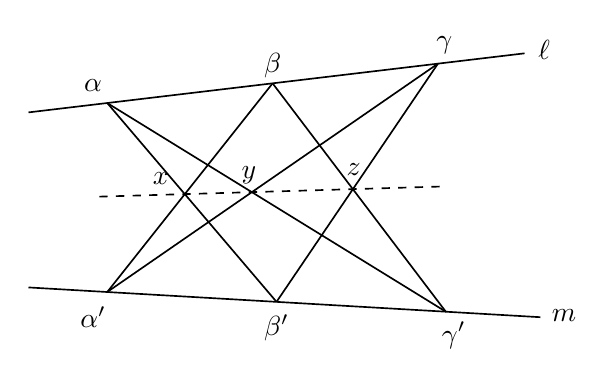
\begin{tikzpicture}[semithick]
  \draw (-1.0,2.281) -- (5.3,3.031);
  \node at (5.55,3.08) {$\ell$};
  \draw (-1.0,0.058) -- (5.5,-0.320);
  \node at (5.8,-0.30) {$m$};
  \draw (0,2.4) -- (2.15,-0.125);
  \draw (0,2.4) -- (4.3,-0.25);
  \draw (2.1,2.65) -- (0,0);
  \draw (2.1,2.65) -- (4.3,-0.25);
  \draw (4.2,2.9) -- (0,0);
  \draw (4.2,2.9) -- (2.15,-0.125);
  \draw[dashed] (-0.10,1.211) -- (4.29,1.341);
  \node at (-0.18,2.62) {$\alpha$};
  \node at (2.1,2.88) {$\beta$};
  \node at (4.28,3.13) {$\gamma$};
  \node at (-0.18,-0.32) {$\alpha'$};
  \node at (2.15,-0.45) {$\beta'$};
  \node at (4.4,-0.55) {$\gamma'$};
  \node at (0.68,1.44) {$x$};
  \node at (1.80,1.48) {$y$};
  \node at (3.13,1.56) {$z$};
\end{tikzpicture}
\caption{\trPappus{}定理。（依原书手绘图重绘。）}\label{fig:pappus}
\end{figure}

\begin{figure}[htbp]
\centering
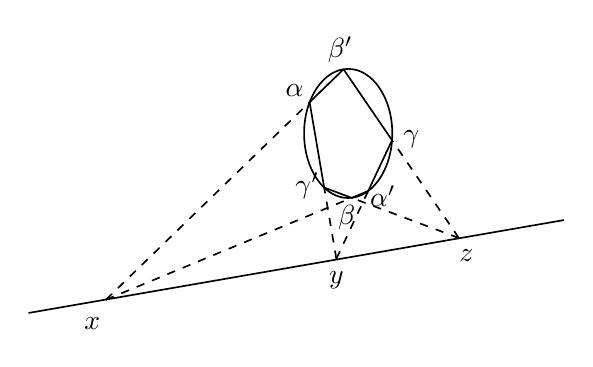
\begin{tikzpicture}[semithick]
  \draw (-4.06,-2.28) -- (2.74,-1.10);
  \draw[dashed] (-3.076,-2.111) -- (-0.490,0.397);
  \draw[dashed] (-3.076,-2.111) -- (0.044,-0.818);
  \draw[dashed] (-0.150,-1.592) -- (-0.305,-0.687);
  \draw[dashed] (-0.150,-1.592) -- (0.254,-0.731);
  \draw[dashed] (1.406,-1.328) -- (0.557,-0.086);
  \draw[dashed] (1.406,-1.328) -- (0.044,-0.818);
  \draw (0,0) ellipse (0.56 and 0.82);
  \draw (-0.490,0.397) -- (-0.305,-0.687);
  \draw (-0.305,-0.687) -- (0.044,-0.818);
  \draw (0.044,-0.818) -- (0.254,-0.731);
  \draw (0.254,-0.731) -- (0.557,-0.086);
  \draw (0.557,-0.086) -- (-0.059,0.815);
  \draw (-0.059,0.815) -- (-0.490,0.397);
  \node at (-0.10,1.06) {$\beta'$};
  \node at (-0.68,0.55) {$\alpha$};
  \node at (0.80,-0.07) {$\gamma$};
  \node at (-0.52,-0.66) {$\gamma'$};
  \node at (0.44,-0.80) {$\alpha'$};
  \node at (-0.02,-1.07) {$\beta$};
  \node at (-3.25,-2.42) {$x$};
  \node at (-0.15,-1.87) {$y$};
  \node at (1.50,-1.55) {$z$};
\end{tikzpicture}
\caption{\trPascal{}的「神秘六边形」定理。（依原书手绘图重绘。）}\label{fig:pascal}
\end{figure}

\textbf{19.4.D.（练习）}\quad 设 $\alpha$、$\beta$、$\gamma$、$\alpha'$、$\beta'$ 是 $\mathbb{P}^2_{\mathbb{R}}$ 中五个点，其中任何三点都不共线。证明：存在唯一的\trConic{} $K$ 经过这五个点。证明 $K$ 是\trRegular{}的。解释如何只用一把直尺（straightedge）构造 $K$ 在 $\alpha$ 处的\trTangentLine。（最后一部分的提示：应用\trPascal{}定理，取 $\gamma'=\alpha$。你或许需要先弄清楚，为什么在这个退化情形下还能应用\trPascal{}定理。）

特别地，给定一个椭圆 $K\subset\mathbb{R}^2$ 与一点 $\alpha\in K$，你现在将能够只用一把直尺构造 $K$ 在 $\alpha$ 处的\trTangentLine。

\textbf{19.4.5.}\ \emph{\mbox{\trPascal{}定理~19.4.4} 的证明。}\quad 我们希望证明：直线 $\overline{xy}$ 与 $\overline{\beta\gamma'}$ 及 $\overline{\beta'\gamma}$ 相交于同一个点。令 $C$ 为由 $K$ 与直线 $\overline{xy}$ 之并所成的曲线。（警告，参看 \S19.2.1：本章仅此一次，我们不假设 $C$ \trRegular！）

令 $D_1$ 为三条直线 $\overline{\alpha\beta'}$、$\overline{\beta\gamma'}$、$\overline{\gamma\alpha'}$ 之并，并令 $D_2$ 为三条直线 $\overline{\alpha'\beta}$、$\overline{\beta'\gamma}$、$\overline{\gamma'\alpha}$ 之并。注意：$D_1$ 与 $C$ 相交于九个点 $\alpha$、$\beta$、$\gamma$、$\alpha'$、$\beta'$、$\gamma'$、$x$、$y$ 以及 $\overline{xy}\cap\overline{\beta\gamma'}$，而 $D_2$ 与 $C$ 相交于同样这九个点，只是其中 $\overline{xy}\cap\overline{\beta\gamma'}$ 换成了 $\overline{xy}\cap\overline{\beta'\gamma}$。于是，倘若我们知道\mbox{推论~19.4.2} 能够适用于我们这条 $C$（它是奇异的），那么就已大功告成（参看\mbox{练习~19.4.C}）。

于是我们把\mbox{推论~19.4.2} 扩充到我们的情形。为此，我们先把\mbox{命题~19.4.1} 扩充到我们的情形。我们有一条平面三次\trCurve{} $C$，它是一条直线 $L$ 与一条\trConic{} $K$ 之并；还有两个点 $p=\overline{xy}\cap\overline{\beta\gamma'}$ 与 $q=\overline{xy}\cap\overline{\beta'\gamma}$，满足 $\OO(p)\cong\OO(q)$。（理由：二者都由 $\OO_{\mathbb{P}^2}(3)$ 限制到 $C$ 上、再经 $-(\alpha+\beta+\gamma+\alpha'+\beta'+\gamma'+x+y)$ 扭转而得。）称这个\trInvertibleSheaf{}为 $\mathscr{L}$。设 $p\ne q$。那么，$\mathscr{L}$ 的在 $p$ 与 $q$ 处取零点的两个截面给出一个\trBasePointFree\trLinearSystem，从而给出一个\trMorphism{} $\pi\colon C\to\mathbb{P}^1$，满足 $\pi^{-1}(0)=p$、$\pi^{-1}(\infty)=q$。

由\mbox{命题~19.4.1} 证明中的论证，$\pi$ 给出 $L$ 与 $\mathbb{P}^1$ 的一个同构。由于 $\pi$ 是\trProper{}的，故 $\pi(K)$ 是闭的；又由于 $K$ \trIrreducible，故 $\pi(K)$ \trIrreducible。由于 $\pi(K)$ 不包含 $0$（或 $\infty$），它不可能是整个 $\mathbb{P}^1$。于是 $\pi(K)$ 是一个点。

这条\trConic{} $K$ 与直线 $L$ 相交于两个点（计重数）——由平面曲线的\trBezout{}定理（\S18.6.4），或由简单的代数可知。若 $K\cap L$ 由两个点 $a$ 与 $b$ 组成，我们便得到矛盾：$K$ 不可能既收缩到 $\pi(a)$ 又收缩到 $\pi(b)$。但如果 $K$ 与 $L$ 相交于一点，也就是说，如果这条\trConic{}与这条直线相切，又会如何？

\textbf{19.4.E.（练习）}\quad 通过处理这个情形来完成\trPascal{}定理的证明。提示：幂零元将前来救场。直观如下：$K\cap L$ 是 $L$ 的一个\trLength{}为 $2$ 的子概形（概形的\trLength{}定义于 \S6.5.8），但可以证明，\trSchemeTheoreticImage{} $\pi(K)$ 是一个\trReduced{}闭点。

\begin{flushright}
$\square$
\end{flushright}

\textbf{19.4.6.}\ \emph{\trhRemark{}。}\quad 作为我们论证之动机的关键事实——\mbox{命题~19.4.1}——核心上是关于\trGenus{}非 $0$ 的\trCurve{}的；然而，\trPappus{}定理与\trPascal{}定理所牵涉的一切\trCurve{}却都具有\trGenus{} $0$。要记在心里的洞见是：\trGenus{} $0$ 的诸\trCurve{}之并未必具有\trGenus{} $0$。在我们的情形中，要紧的是三次\trCurve{}具有\trGenus{} $1$，哪怕它们是若干个 $\mathbb{P}^1$ 的并。
